\section{Evaluation Plan and Timeline}
\label{sec:evaluation}

\noindent \textit{\textbf{Prototype.}} We will target Intel CPUs for our prototypes due to our prior experience. We will extend Apport~\cite{ubuntuApport} clients to receive server commands and relay to the Intel PT driver (T1.1). On the server side, we will rely on S2E~\cite{Chipounov11} for symbolic execution (T1.1, T1.3, T2.3), which translates QEMU~\cite{qemu} microcode to LLVM to use Klee as a backend for symbolic execution. Unlike Klee, S2E supports native binaries and does not require an environment model (e.g., of the OS). Our work on whole-program analysis~\cite{snorlax} and data race detection~\cite{portend} will inform hybrid slicing and concurrency bug detection (T1.2, T2.1). We will use the timestamp monitoring support from our prior work~\cite{snorlax} to implement schedule refinement (T2.2). \textit{All the techniques will be composed into a final prototype, which will be released openly}.

\noindent \textit{\textbf{Metrics.}} We will use the metrics from \S\ref{sec:related}: (1) Effectiveness, is the percentage of bugs reproduced, (2) Accuracy is the percentage of data and control information that is reconstructed correctly for reproduced bugs, (3) Efficiency is the runtime or throughput overhead over native execution, (4) Non-invasiveness is the percentage of code that is added to a system to enable bug reproduction. We will also use (5) Bug Reproduction Latency, which is the time it takes to reproduce a bug after it has occurred.


\noindent \textit{\textbf{Evaluation Targets and Methodology.}} We will pursue a 2-pronged evaluation to assess how our \textit{end-to-end} bug reproduction system fares in light of the above metrics. First, we will use our corpus of 510 real-world bugs (\S\ref{sec:preliminary}), which includes bugs used in related work~\cite{jieyucon28:database,lin:jacontebe,snorlax,gist}. Second, we will port our prototype to Windows (e.g., through internships and technology transfer) and evaluate it at REPT's~\cite{rept} global scale (see letter from Dr. Cui). \textit{This is crucial since we will assess how our techniques fare in the real world and improve upon the state-of-the-art (i.e., REPT)}. Besides the end-to-end evaluation, we will determine the individual and combined contributions of each technique to the metrics. We will also evaluate the effects of optimizations (e.g., How much do hybrid slices simplify static slices and speed up symbolic execution?, How much do the core dump and schedule simplification speed up symbolic execution? How much does schedule refinement reduce the interleavings to explore; How effective clock amplification is in identifying happens-before relationships? Finally, for all tunable parameters, we will carry out a detailed sensitivity analysis. (e.g., How do the evaluation metrics vary with the various trace buffer sizes (besides the default 1MB) used for control flow and data flow tracking?)

\begin{wraptable}{l}{50mm}
    \caption{Research Plan}
    \label{table:plan}
    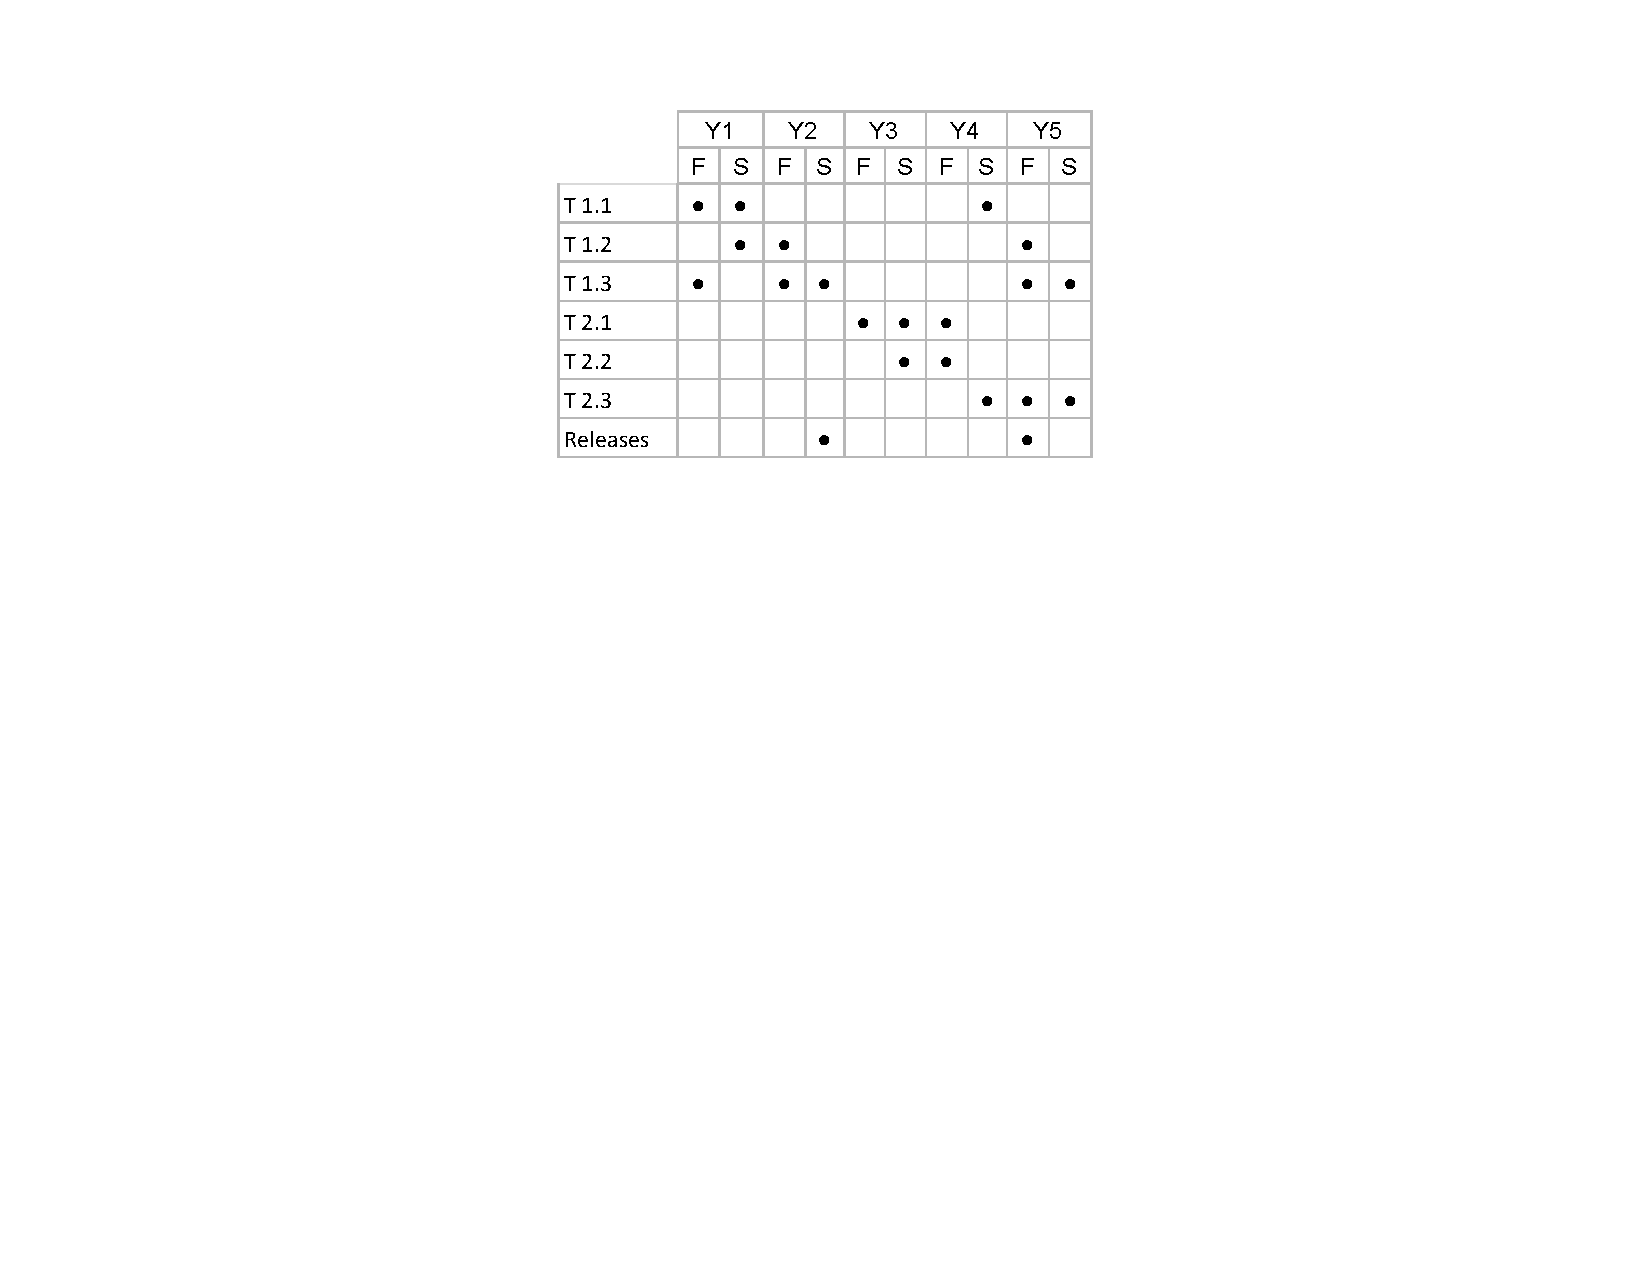
\includegraphics[width=\linewidth]{Figures/plan.pdf}
\end{wraptable}

\noindent \textit{\textbf{Timeline.}} In Table~\ref{table:plan}, years are split into a (F)irst and (S)econd half. In Y1, we will build the trace-driven symbolic execution engine (T1.1) and start with hybrid slice computation (T1.2) and adaptive symbolic execution (T1.3), both of which will continue in Y2. In Y2, we will build the Execution Reconstruction prototype and submit the paper to SOSP. In Y3, we will focus on hybrid concurrency bug detection (T2.1) and start schedule refinement (T2.2), which will continue in Y4. In Y4, we will start implementing symbolic schedule synthesis (T2.3) and add time tracking to trace-driven symbolic execution (T1.1). Y5 will integrate all the techniques, mainly adaptive symbolic execution and symbolic schedule synthesis. We will submit the Execution Stitching paper to OSDI. 

\noindent \textit{\textbf{Risk Mitigation.}} Thrust 2 can be decoupled from Thrust 1 to mitigate delays. We can build many techniques and concepts atop the S2E symbolic execution engine and achieve good metrics besides efficiency.

\noindent \textit{\textbf{Success Criteria}} Our primary success criterion is outperforming all existing bug reproduction techniques but record/replay across all metrics. Our second criterion is to perform at 90\% and above of the effectiveness and accuracy of record/replay systems, while being orders of magnitude more efficient. We target overheads of 1-3\%, which we achieved in prior work~\cite{rept,snorlax}.

\noindent \textit{\textbf{Effort and Budget.}} The bulk of the budget will support a graduate student for 5 years as well as some undergraduates that will assist in building the fully reproducible real-world bug framework.

